\subsection{Reducers to constrain ring colorings}
\label{sec:reducers}

As we have seen in the reducibility proof of $R_4$, we had enough guaranteed colorings to find a common ring coloring through the reconfiguring of schemes. However, as we will see in the next section, we will need guaranteed 3-colorings like $cabab$ and $abcab$ to prove that configurations on $R_5$ are reducible. A 3-coloring is not guaranteed from simply contracting ring vertices from Theorem \ref{thm:ringsarered}. Therefore, we seek a technique to obtain more guaranteed colorings such as 3-colorings.

However, such a technique will come at cost. The cost is that we will no longer be able to reduce to $M+R$, and must instead reduce to a slightly bigger graph $M+S$ where $R \subset S$. The graph $S$ is called a \textit{reducer}. It is chosen in such a way that it guarantees the colorings we need in $\Phi(M+S)$. The reducer that we will use to guarantee 3-colorings of $R_5$ is shown in Figure \ref{fig:reducertut}.

\begin{figure}[!h]
    \centering
    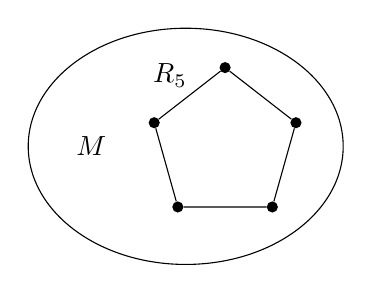
\begin{tikzpicture}
        \draw[fill=white] (-0.5, 0) ellipse (2cm and 1.5cm);
        \node at (-1.7, 0) {$M$};
        \node at (-0.7, 0.9) {$R_5$};

        \node[circle, fill, scale=0.015cm] (l1) at (0, 1) { };
        \node[circle, fill, scale=0.015cm] (l2) at (0.9, 0.30) { };
        \node[circle, fill, scale=0.015cm] (l3) at (0.6, -0.77) {};
        \node[circle, fill, scale=0.015cm] (l4) at (-0.6, -0.77) {};
        \node[circle, fill, scale=0.015cm] (l5) at (-0.9, 0.30) {};

        \draw (l1) -- (l2) -- (l3) -- (l4) -- (l5) -- (l1);
    \end{tikzpicture}
    \hspace{1cm}
    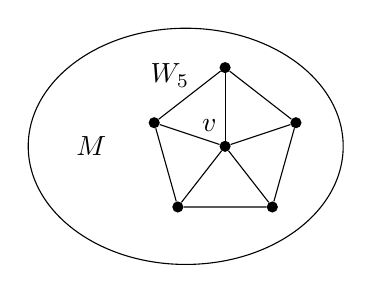
\begin{tikzpicture}
        \draw[fill=white] (-0.5, 0) ellipse (2cm and 1.5cm);
        \node at (-1.7, 0) {$M$};
        \node at (-0.7, 0.9) {$W_5$};

        \node (c) at (-0.2, 0.27) { $v$ };
        \node[circle, fill, scale=0.015cm] (c) at (0, 0) {};
        \node[circle, fill, scale=0.015cm] (l1) at (0, 1) { };
        \node[circle, fill, scale=0.015cm] (l2) at (0.9, 0.30) { };
        \node[circle, fill, scale=0.015cm] (l3) at (0.6, -0.77) {};
        \node[circle, fill, scale=0.015cm] (l4) at (-0.6, -0.77) {};
        \node[circle, fill, scale=0.015cm] (l5) at (-0.9, 0.30) {};

        \draw (c) -- (l1);
        \draw (c) -- (l2);
        \draw (c) -- (l3);
        \draw (c) -- (l4);
        \draw (c) -- (l5);
        \draw (l1) -- (l2) -- (l3) -- (l4) -- (l5) -- (l1);
    \end{tikzpicture}
    \caption{The graph $M+R_5$ (left). The graph $M+W_5$ that guarantees 3-colorings of the $R_5$ (right).}
    \label{fig:reducertut}
\end{figure}

The reduction we used for $R_4$ is similar to the left-most graph in Figure \ref{fig:reducertut}. This graph allows us to contract two vertices of the $R_5$ to force them to be the same color. Since there are 5 ways to contract two non-neighboring vertices of $R_5$, we are guaranteed all of the following 5 colorings.

\begin{equation}
    \Phi^\star(5) = \{ a{*}{*}a{*}, \quad {*}a{*}{*}a, \quad a{*}a{*}{*}, \quad {*}a{*}a{*}, \quad {*}{*}a{*}a \}.
\end{equation}

The ${*}$-colors in these colorings are still unknown. This set $\Phi^\star(5)$ contains all the guaranteed colorings from contracting vertices of the ring $R_5$. Every ring has such a set. For the ring reducibility proof of $R_4$ for example, we used the following set of 2 colorings.

\begin{equation}
    \Phi^\star(4) = \{ a{*}a{*}, \; {*}a{*}a \}.
\end{equation}

\begin{definition}
    The set $\Phi^\star(n)$ consists of all guaranteed ${*}$-colorings of $R_n$ obtained from successive contraction of non-neighboring vertices.
\end{definition}

Imagine how larger rings like $R_6$ are able to contract two opposing vertices twice in a row. This guarantees that 2 pairs of vertices are colored the same. We wont be using these sets for rings beyond $R_5$, but it should not be difficult to define exactly all the ${*}$-colorings for every ring $R_n$.

To continue with our introduction of reducers, let us consider now the colorings of the right-most graph $M+W_5$ in Figure \ref{fig:reducertut}. The graph $S=W_5$ is called the \textit{wheel graph} on $R_5$. It is clear that this graph is 1 vertex bigger than $M+R_5$, hence making it a weaker reduction. However, in exchange we are guaranteed \textit{only one} of the following five 3-colorings.

\begin{equation}
    \Phi^{W_5} = \{ \underline{c}abab\;\;\lor\;\; 
            a\underline{c}bab\;\;\lor\;\;
            ab\underline{c}ab\;\;\lor\;\;
            aba\underline{c}b\;\;\lor\;\;
            abab\underline{c} \}.
\end{equation}

We have underlined the uniquely colored vertex of each 3-coloring. From the usage of a logical-OR symbol $(\lor)$, we will have in fact multiple options for the set $\Phi^{W_5}$. In general, we will use the notation $\Phi^S$ to indicate \textit{some} set of guaranteed ring colorings of a reducer $S$, even if there are multiple options for this set.

\begin{definition}
    The set $\Phi^S$ is \emph{some} set of guaranteed ring colorings of a reducer $S$.
\end{definition}

From the examples of the sets $\Phi^\star(5)$ and $\Phi^{W_5}$, it is clear that the use of a reducer guarantees more types of ring colorings. These guarantees can then be used to find common ring colorings of two graphs, through the reconfiguration of Kempe-chains. Therefore, let the reduction for $M$ be given by

\begin{equation}
    M+S \;\;  \text{with} \;\; R_n \subset S \;\; \text{and} \;\; |S| \leq k+n.
\end{equation}

The $k$ in the maximum size of our reducer $|S| \leq k+n$ indicates how many other vertices we have in $S$ besides the ring $R_n$. This parameter determines the amount of \textit{control} we have over the ring colorings. 

\begin{itemize}
    \item If $k=0$ we can take $R_4$ as example. In this case we had $S=R_4$ and we reduced to $M+R_4$. This is the smallest possible reduction. We could only use guaranteed colorings in $\Phi^\star(4)$.
    
    \item If $k=1$, we can take $R_5$ as example. Here we will set $S=W_5$ such that we reduce to $M+W_5$ instead. This gives us a guaranteed 3-coloring from $\Phi^{W_5}$. However, the graph $M+W_5$ would only be smaller than $M+\confg$ if $\confg > W_5$. This means that there must be at least 2 vertices in the interior of $\confg$. This limits which configurations on $R_5$ are reducible.
    
    \item If $k \geq |\confg|$, then there is never a point in reducing, since we always obtain the same graph $M+\confg$ by setting $S=\confg$ or a larger one. 
\end{itemize}

Therefore, we must require that $k < \confg$ in order for $\confg$ to be reducible. With this, all the components to define $k$-reducibility of a configuration $\confg$ are in place.

\begin{definition}
    A configuration $\confg$ on $R_n$ is $k$-\emph{reducible} for $k < |\confg|$, if for all planar graphs $M$ there exists a reducer with $|S| \leq k$ such that
    \begin{equation}
        \Phi(M+S)\; \cap\; \Phi(\confg) \quad \neq  \quad\varnothing.
    \end{equation}
\end{definition}

We have already proven that configurations on $R_4$ are 0-reducible. Configurations on $R_1, R_2$ and $R_3$ are also trivial examples of 0-reducibility. Their only colorings are of the form $a$, $ab$ and $abc$ respectively, therefore, we have $\Phi(M+R_n) = \Phi(\confg)$ for each of them. We have hinted a non-trivial example in our motivation for reducers. This is where we prove the 1-reducibility of configurations on $R_5$. 